\documentclass[]{article}
\usepackage[brazil]{babel}
\usepackage{graphicx}
\usepackage{mathtools}
\usepackage{float} 
\usepackage{xcolor}
\usepackage{amsmath}
\usepackage{xcolor}
\usepackage{hyperref}

\usepackage{array}
\usepackage{booktabs}



% margenes
\usepackage[a4paper,left=3cm,right=3cm,top=3cm]{geometry}

%opening
\title{}
\author{}

\begin{document}
	
\begin{center}
	{\tiny {\normalsize {\large Trabalho de Cavidade com tampa deslizante\\
				Transferência de calor e mecânica dos fluidos computacional I\\
				\textbf{Cristian Herledy Lopez Lara}}}}
\end{center}


\section*{Introdução}
O exercício de cavidade de trampa deslizante é um problema bem conhecido no desenvolvimento de ferramentas computacionais para modelar matematicamente os problemas físicos de mecânica dos fluidos e transferência de calor. Para este artigo, sua aplicação visa compreender e utilizar um modelo matemático que resolve numericamente o campo de velocidade e temperatura como efeito do movimento do fluido e da transferência de calor dentro das paredes da cavidade. Neste exercício, analisaremos como o fluxo se comporta em função de vários números de Reynolds, utilizando equações de conservação de massa, momento e energia, para um caso bidimensional incompressível. Além disso, o desenvolvimento deste trabalho servirá para testar as habilidades para descrever os fenômenos do movimento de fluidos e resolver o problema numérico.

Ao aplicar o método dos volumes finitos, as equações governantes são discretizadas e limitadas com condições de contorno, e então um acoplamento de pressão e velocidade é implementado em um código de solução numérica. Diferentes discretizações e velocidades espaciais são testadas para ver o efeito no fluxo.

\section*{Discretização das Equações Governantes discretização}

Este problema foi simplificado assumindo propriedades de fluido constantes como $k, Cp, \rho$ e $\mu$. As equações diferenciais para a conservação da massa, momento e energia na sua forma conservativa suportam o modelo matemático que deve ser resolvido discretamente para obter os campos de velocidade, pressão e subsequentemente temperatura.\\
	
Equação para balanço de massa
\begin{equation}
	\begin{aligned}
		\frac{\partial \rho}{\partial t} + \frac{\partial}{\partial x}(\rho u) + \frac{\partial}{\partial x}(\rho v) = 0
	\end{aligned}
	\label{eq:1}	
\end{equation}\\

Equações para balanço de cantidad de movimiento (NS-x)\\
Na direção x
\begin{equation}
	\begin{aligned}
		\frac{\partial \rho u}{\partial t} + \frac{\partial}{\partial x}(\rho uu) + \frac{\partial}{\partial x}(\rho vu) = \dfrac{\partial}{\partial x}(\mu\dfrac{\partial u}{\partial x}) + \dfrac{\partial}{\partial y}(\mu\dfrac{\partial u}{\partial y}) -\frac{\partial P}{\partial x}
	\end{aligned}
	\label{eq:2}	
\end{equation}\\

Equação para balanço de cantidad de movimiento (NS-y)\\
Na direção y
\begin{equation}
	\begin{aligned}
		\frac{\partial \rho v}{\partial t} + \frac{\partial}{\partial x}(\rho uv) + \frac{\partial}{\partial x}(\rho vv) = \dfrac{\partial}{\partial x}(\mu\dfrac{\partial v}{\partial x}) + \dfrac{\partial}{\partial y}(\mu\dfrac{\partial v}{\partial y}) -\frac{\partial P}{\partial y}
	\end{aligned}
	\label{eq:3}	
\end{equation}\\

Equação para balanço de energia para o problema de transferência de calor
 
\begin{equation}
	\begin{aligned}
		\frac{\partial \rho T}{\partial t} + \frac{\partial}{\partial x}(\rho uT) + \frac{\partial}{\partial x}(\rho vT) = \dfrac{\partial}{\partial x}(\frac{k}{Cp} \dfrac{\partial T}{\partial x}) + \dfrac{\partial}{\partial y}(\frac{k}{Cp}\dfrac{\partial T}{\partial y})
	\end{aligned}
	\label{eq:4}	
\end{equation}\\

As equações anteriores, que descrevem a conservação da massa, cantidade de movimiento e energia para o problema a ser resolvido, podem ser escritas de forma geral para uma variável $\phi$ como

\begin{equation}
	\begin{aligned}
		\frac{\partial \rho \phi}{\partial t} + \frac{\partial}{\partial x}(\rho u\phi) + \frac{\partial}{\partial x}(\rho v\phi) = \dfrac{\partial}{\partial x}(\varGamma^{\phi} \dfrac{\partial \phi}{\partial x}) + \dfrac{\partial}{\partial y}(\varGamma^{\phi} \dfrac{\partial \phi}{\partial y}) + S^{\phi}
	\end{aligned}
	\label{eq:5}	
\end{equation}\\

Onde os termos associados à variável para cada equação de conservação assumem os seguintes valores:\\
Para conservação de Balanço de massa: 
\begin{equation*}
		\phi = 1 ; \varGamma^{\phi} = 0 ; S^{\phi} = 0 
\end{equation*}\\
Para conservação de Balanço de movimiento em x: 
\begin{equation*}
	\phi = u ; \varGamma^{\phi} = \mu ; S^{\phi} =  -\frac{\partial P}{\partial x}
\end{equation*}\\
Para conservação de Balanço de movimiento em y: 
\begin{equation*}
	\phi = v ; \varGamma^{\phi} = \mu ; S^{\phi} =  -\frac{\partial P}{\partial y}
\end{equation*}\\
Para conservação de Balanço de energia: 
\begin{equation*}
	\phi = T ; \varGamma^{\phi} = \frac{k}{Cp} ; S^{\phi} =  0
\end{equation*}\\

Aplicando a técnica de utilização de volumes finitos para integrar as equações governantes na sua forma conservativa sobre um volume elementar e obter as equações aproximadas que satisfazem as três conservações. O referido volume elementar é definido como P, com as convenções e discretização espacial conforme segue na figura a seguir.

\begin{figure}[H]
	\centering
	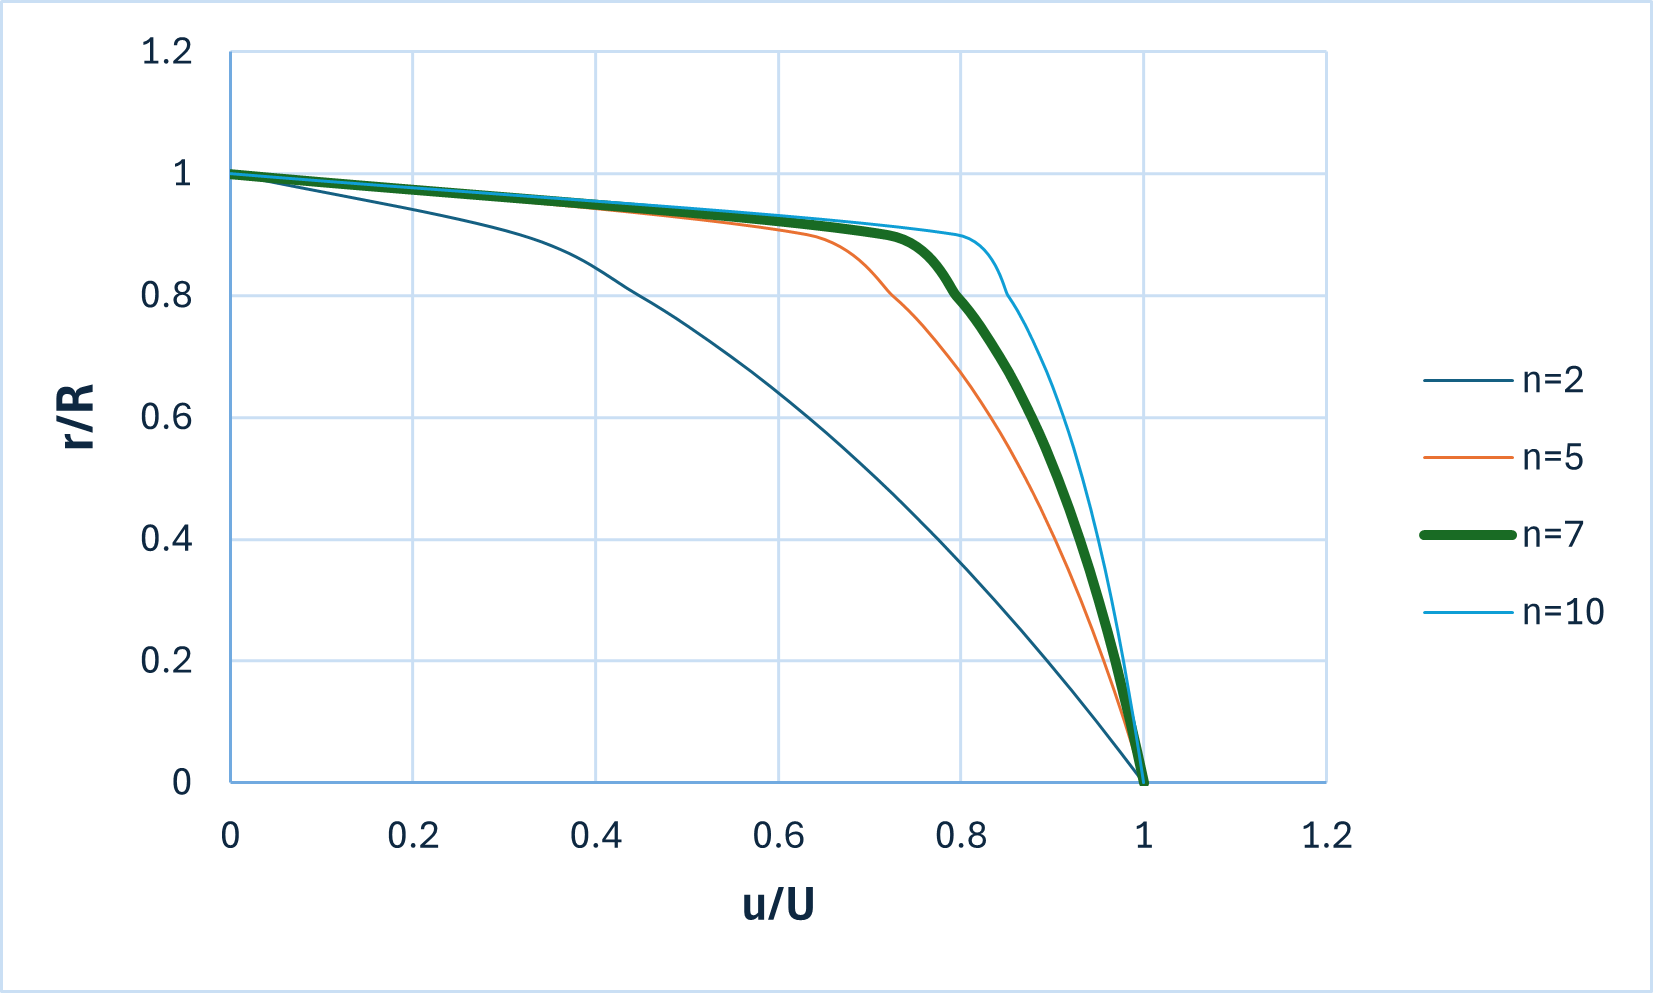
\includegraphics[width=.65\textwidth]{figures/1}
	\caption{Volumen elementar P con nodos e volumes vizinhos}
\end{figure}

O sistema cartesiano com coordenadas norte, sul, leste e oeste será utilizado para melhor compreensão do espaço nas equações a serem discretizadas.

Utilizando a forma da equação \eqref{eq:5}, é possível fazer mais facilmente sua integração espacial e temporal sobre P para o problema acoplado das equações \eqref{eq:1} a \eqref{eq:4}. Integrando a equação 5 obtemos

\begin{equation}
	\begin{aligned}
		\int_{V,t}\frac{\partial \rho \phi}{\partial t} dVdt + \int_{V,t}\frac{\partial}{\partial x}(\rho u\phi) dVdt + \int_{V,t}\frac{\partial}{\partial x}(\rho v\phi) dVdt =\\ \int_{V,t}\dfrac{\partial}{\partial x}(\varGamma^{\phi} \dfrac{\partial \phi}{\partial x}) dVdt + \int_{V,t}\dfrac{\partial}{\partial y}(\varGamma^{\phi} \dfrac{\partial \phi}{\partial y}) + \int_{V,t}S^{\phi} dVdt
	\end{aligned}
	\label{eq:5}	
\end{equation}\\

Usando a equação de interpolação de tempo $\phi^{\theta} = \theta\phi + (1-\theta)\phi^{0}$, fica 

\begin{equation}
	\begin{aligned}
		\frac{\rho \Delta x \Delta y }{\Delta t}\phi_{p} - \frac{\rho \Delta x \Delta y }{\Delta t}\phi_{p}^{0} + \rho u \Delta y\arrowvert_{e} \phi_{e}^{\theta} - \rho u \Delta y\arrowvert_{w}\phi_{w}^{\theta}  + \rho v \Delta x\arrowvert_{n}\phi_{n}^{\theta}  - \rho v \Delta y\arrowvert_{s}\phi_{s}^{\theta}  =\\
		\varGamma^{\phi}\frac{\partial \phi}{\partial x}|_{e}^{\theta}\Delta y - 
		\varGamma^{\phi}\frac{\partial \phi}{\partial x}|_{w}^{\theta}\Delta y + 
		\varGamma^{\phi}\frac{\partial \phi}{\partial y}|_{n}^{\theta}\Delta x - 
		\varGamma^{\phi}\frac{\partial \phi}{\partial y}|_{s}^{\theta}\Delta x + (Sp\phi_{p}^{\theta} + Sc)\Delta x \Delta y
	\end{aligned}		
\end{equation}\\

Substituindo os coeficientes de fluxo de massa e de difusão por

\begin{equation*}
	\begin{aligned}
		M_e = \rho u \Delta y\arrowvert_{e} ; M_w = \rho u \Delta y\arrowvert_{w} ; M_n = \rho v \Delta x\arrowvert_{n} ; M_s = \rho v \Delta x\arrowvert_{s}
	\end{aligned}		
\end{equation*}

\begin{equation*}
	\begin{aligned}
		D_e = \varGamma^{\phi} \Delta y\arrowvert_{e} ; D_w = \varGamma^{\phi} \Delta y\arrowvert_{w} ; D_n = \varGamma^{\phi} \Delta x\arrowvert_{n} ; D_s = \varGamma^{\phi} \Delta x\arrowvert_{s}
	\end{aligned}		
\end{equation*}\\
\begin{equation*}
	\begin{aligned}
		M_P = \frac{\rho \Delta x \Delta y }{\Delta t}
	\end{aligned}		
\end{equation*}\\

Fica

\begin{equation}
	\begin{aligned}
		M_P\phi_{p} - M_P\phi_{p}^{0} + M_e\phi_{e}^{\theta} - M_w\phi_{w}^{\theta}  + M_n\phi_{n}^{\theta}  - M_s\phi_{s}^{\theta}  =\\
		D_e\frac{\partial \phi}{\partial x}|_{e}^{\theta} - 
		D_w\frac{\partial \phi}{\partial x}|_{w}^{\theta} + 
		D_n\frac{\partial \phi}{\partial y}|_{n}^{\theta} - 
		D_s\frac{\partial \phi}{\partial y}|_{s}^{\theta} + Sp\phi_{p}^{\theta}\Delta x \Delta y + Sc\Delta x \Delta y
	\end{aligned}		
\end{equation}\\


\subsection*{Condições de Contorno}


\subsection*{Fronteira Superior (\(y = h\))}
\begin{itemize}
	\item Velocidade: Dirichlet prescrita
	\[
	u = U, \quad v = 0
	\]
	
	\item Temperatura: Dirichlet prescrita
	\[
	T = 2
	\]
	
\end{itemize}

\subsection*{Fronteira Inferior (\(y = 0\))}
\begin{itemize}
	\item Velocidade: Dirichlet prescrita 
	\[
	u = 0, \quad v = 0
	\]
	
	\item Temperatura: Dirichlet prescrita
	\[
	T = 1
	\]
	
\end{itemize}

\subsection*{Fronteira Izquierda (\(x = 0\))}
\begin{itemize}
	\item Velocidade: Dirichlet prescrita
	\[
	u = 0, \quad v = 0
	\]
	
	\item Temperatura: Dirichlet prescrita
	\[
	T = 1
	\]
	
\end{itemize}

\subsection*{Frontera Derecha (\(x = h\))}
\begin{itemize}
	\item Velocidade: Dirichlet prescrita 
	\[
	u = 0, \quad v = 0
	\]
	
	\item Temperatura: Dirichlet prescrita
	\[
	T = 1
	\]
	
\end{itemize}

Empregando a função de interpolação do esquema WUDS, para os termos advectivos

\begin{equation}
	\begin{aligned}
		\phi_e &= \left( \frac{1}{2} + \alpha_e \right) \phi_P + \left( \frac{1}{2} - \alpha_e \right) \phi_E \\
		\phi_w &= \left( \frac{1}{2} + \alpha_w \right) \phi_P + \left( \frac{1}{2} - \alpha_w \right) \phi_W \\
		\phi_n &= \left( \frac{1}{2} + \alpha_n \right) \phi_P + \left( \frac{1}{2} - \alpha_n \right) \phi_N \\
		\phi_s &= \left( \frac{1}{2} + \alpha_s \right) \phi_P + \left( \frac{1}{2} - \alpha_s \right) \phi_S \\
	\end{aligned}		
\end{equation}\\

Para os termos difusivos

\begin{equation}
	\begin{aligned}
		\Gamma^\phi \left( \frac{\partial \phi}{\partial x} \right)_e &=  \Gamma_e^\phi \left( \frac{\phi_E - \phi_P}{\Delta x} \right) \\
		\Gamma^\phi \left( \frac{\partial \phi}{\partial x} \right)_w &=  \Gamma_w^\phi \left( \frac{\phi_P - \phi_W}{\Delta x} \right) \\
		\Gamma^\phi \left( \frac{\partial \phi}{\partial y} \right)_n &=  \Gamma_n^\phi \left( \frac{\phi_N - \phi_P}{\Delta y} \right) \\
		\Gamma^\phi \left( \frac{\partial \phi}{\partial y} \right)_s &=  \Gamma_s^\phi \left( \frac{\phi_P - \phi_S}{\Delta y} \right)
	\end{aligned}		
\end{equation}\\

E adicionando a equação de conservação de massa

\begin{equation}
	\frac{M_P - M_P^\circ}{\Delta t} + M_e - M_w + M_n - M_s = 0
\end{equation}

Obtemos

\begin{equation}
	\begin{aligned}
		\frac{M_P}{\Delta t} \phi_P + A_P \phi_P &= A_E \phi_E + A_W \phi_W + A_S \phi_S + A_N \phi_N + A_F \phi_F + A_B \phi_B + \frac{M_P}{\Delta t} \phi_P + Sc \Delta V \\
		A_P &= A_E + A_W + A_N + A_S + A_F + A_B - S_P \Delta V - \frac{M_P}{\Delta t} + \frac{M_P^\circ}{\Delta t} \\
		A_E &= \left( \frac{1}{2} - \alpha_E \right) M_e + D_e  \left( \frac{1}{\Delta x} \right) |_e \\
		A_W &= \left( \frac{1}{2} + \alpha_W \right) M_w + D_w \left( \frac{1}{\Delta x} \right) |_w \\
		A_N &= \left( \frac{1}{2} - \alpha_N \right) M_n + D_n  \left( \frac{1}{\Delta y} \right) |_n \\
		A_S &= \left( \frac{1}{2} + \alpha_S \right) M_s + D_s  \left( \frac{1}{\Delta y} \right) |_s
	\end{aligned}
\end{equation}
Onde o coeficiente $\alpha$ é calculado em termos do número de Peclet.

Devido às não linearidades nas equações de momento, o sistema de equações descrito requer um acoplamento entre pressão e velocidade para sua solução.

O esquema de arranjo desencontrado fue escogido para la lozalizacion de las variables para posicionar los vectores de velocidad y la presion. La presion es situada en el centro del volumen de control, y la velocidad calculada en las caras, donde para el calculo del acoplamiento se evalua la conservacion en volumenes adicionales



\subsection*{Determinação do campo de velocidade}
O sistema de equações descrito pode ser escrito da seguinte maneira

\begin{equation}
	A_P U_P = A_E u_E + A_W u_W + A_N u_N + A_S u_S - L \left[ P^u \right] \Delta V + B_P
\end{equation}

\begin{equation}
	A_P V_P = A_E v_E + A_W v_W + A_N v_N + + A_S v_S - L \left[ P^v \right] \Delta V + B_P 
\end{equation}

Em que $\phi$ é substituído pela variável a ser considerada para a conservação da massa e do momento. O problema agora é resolver estas equações para obter o campo de velocidades, que como se sabe tem um problema de não linearidade implícito.\\

Neste exercício optou-se por utilizar o método da solução segregada juntamente com o porta-enxerto não encontrado como se vê na figura seguinte.

\begin{figure}[H]
	\centering
	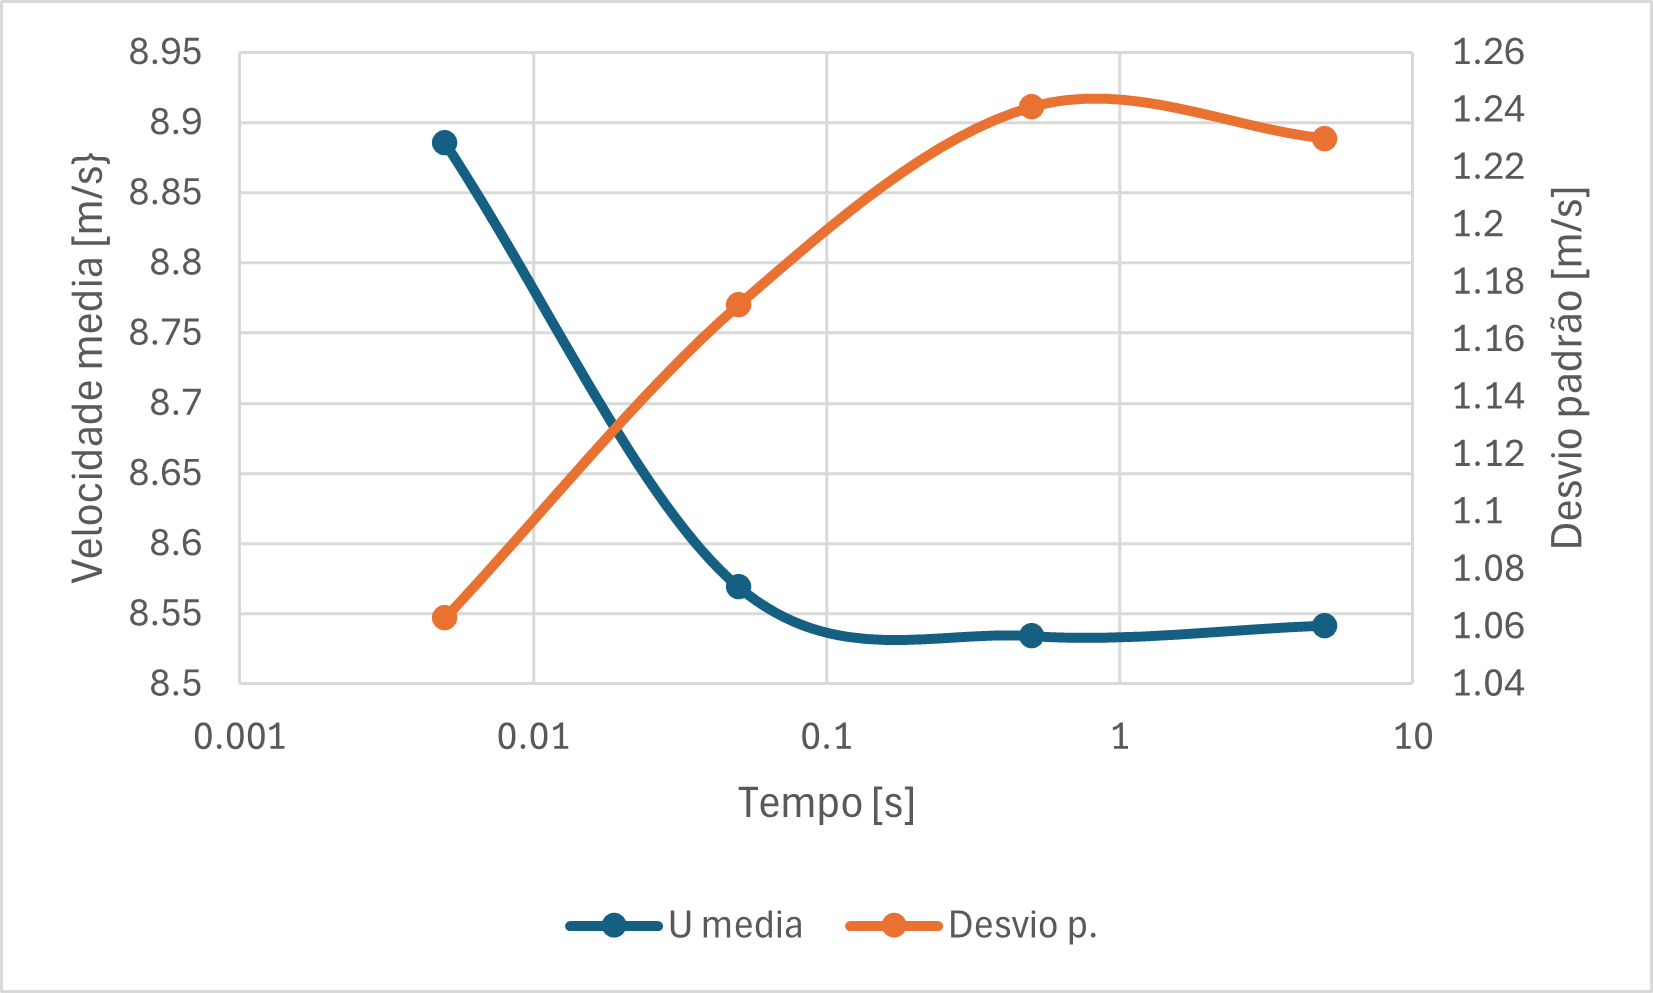
\includegraphics[width=.65\textwidth]{figures/2}
	\caption{Diagrama de arranjo desencontrado}
\end{figure}

Para o acoplamento pressão-velocidade, optou-se pela utilização do método SIMPLE. Adicionando um campo de pressão P* nas equações 13 e 14,

\begin{equation}
	A_P u_P^{*} = A_E u_E^{*} + A_W u_W^{*} + A_N u_N^{*} + A_S u_S^{*} - L \left[ P^u \right]^{*} \Delta V + B_P
\end{equation}

\begin{equation}
	A_P v_P^{*} = A_E v_E^{*} + A_W v_W^{*} + A_N v_N^{*} + A_S v_S^{*} - L \left[ P^v \right]^{*} \Delta V + B_P 
\end{equation}


Quando o campo de pressão inserido está correto, podemos encontrar as seguintes expressões para a correção das velocidades

\begin{equation}
	u_P = u_P^* - \frac{\Delta V}{A_P} \frac{\Delta P'}{\Delta x}\\;
	v_P = v_P^* - \frac{\Delta V}{A_P} \frac{\Delta P'}{\Delta y}
\end{equation}

Que quando escrito para fazer uso da conservação da massa, obtemos as equações para obter $P'$ a assim

\begin{equation}
	u_e = u_e^* - d_e^u \left( P_E' - P_P' \right)
\end{equation}

\begin{equation}
	u_w = u_w^* - d_w^u \left( P_P' - P_W' \right)
\end{equation}

\begin{equation}
	v_n = v_n^* - d_n^\nu \left( P_N' - P_P' \right)
\end{equation}

\begin{equation}
	v_s = v_s^* - d_s^\nu \left( P_P' - P_S' \right)
\end{equation}

Usando a equação de conservação de massa, obtemos uma equação discretizada para $P'$ da forma

\begin{equation}
	A_P P_P' = A_e P_E' + A_w P_W' + A_s P_S' + A_n P_N' + A_f P_F' + A_b P_B' - \nabla \cdot \mathbf{V}^*
\end{equation}\\

Uma vez corrigidas as velocidades, a pressão é obtida com

\begin{equation}
	P = P^{*} + P'
\end{equation}

Como a equação não possui um suporte físico forte, ela é deduzida usando a equação de conservação da massa. Por esta razão, um coeficiente de relaxação deve ser utilizado tal que

\begin{equation}
	P = P^{*} + \alpha P'
\end{equation}


\section*{Resultados}

Este trabalho foi realizado para resolver o problema da cavidade da tampa deslizante com dimensões de LxW = 1x1, utilizando sistemas de discretização espacial e acoplamento pressão-velocidade em regime laminar $(100 < Re < 100)$. O problema foi resolvido assumindo um fluido incompressível, com estudo computacional de diferentes refinamentos de malha e valores de número de Reynolds.\\

Os resultados serão comparados com o trabalho realizado por \textbf{Ghia, 1982}[3]; Este trabalho é de importância no campo da mecânica dos fluidos porque tem servido como guia para testar solucionadores computacionais.\\

Issos resultados obtidos serão apresentados para malhas computacionais de 10x10, 20x20, 50x50 e um caso de 100 x 100 (devido à disponibilidade do recurso computacional). Essas malhas serviram de espaço para testar fluxos de Re = 100, 500 e 1000. A comparação com o trabalho de Ghia foi feita através da obtenção dos valores de velocidade em uma linha vertical em x = 0,5. 

\subsection*{Casos para o numero de Reynolds Re=100}


\begin{figure}[H]
	\centering
	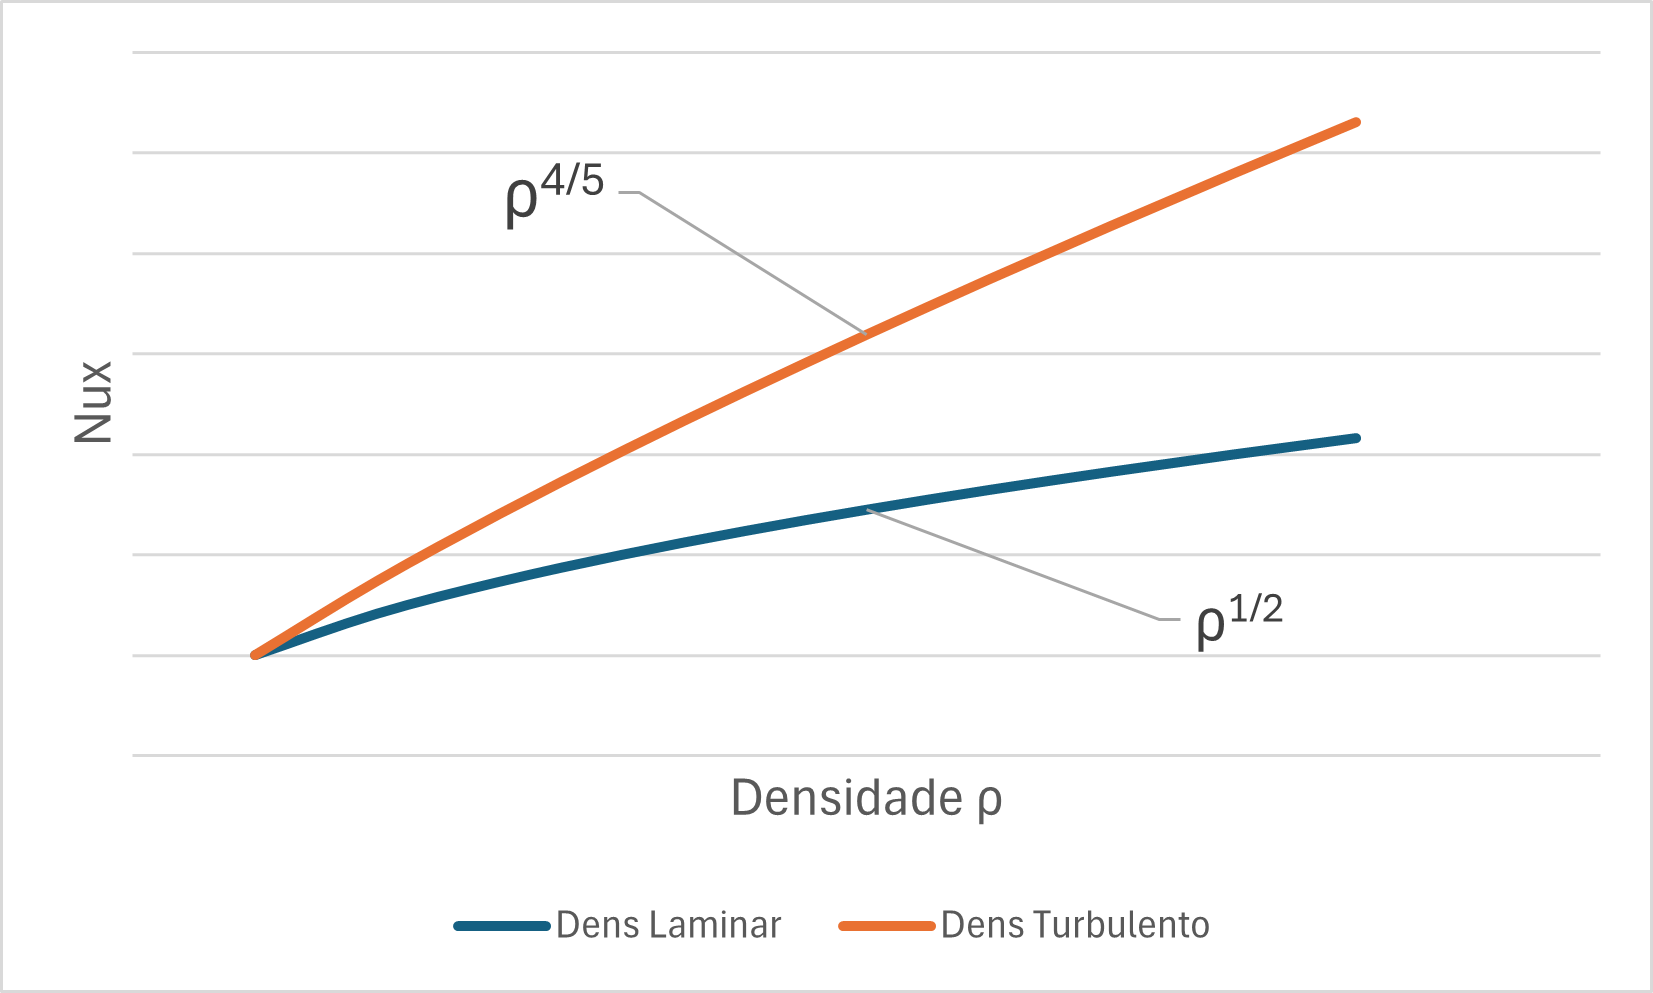
\includegraphics[width=.65\textwidth]{figures/3}
	\caption{Distribuição de $u$ em x = 0,5 malha 10x10 volumes}
\end{figure}

\begin{figure}[H]
	\centering
	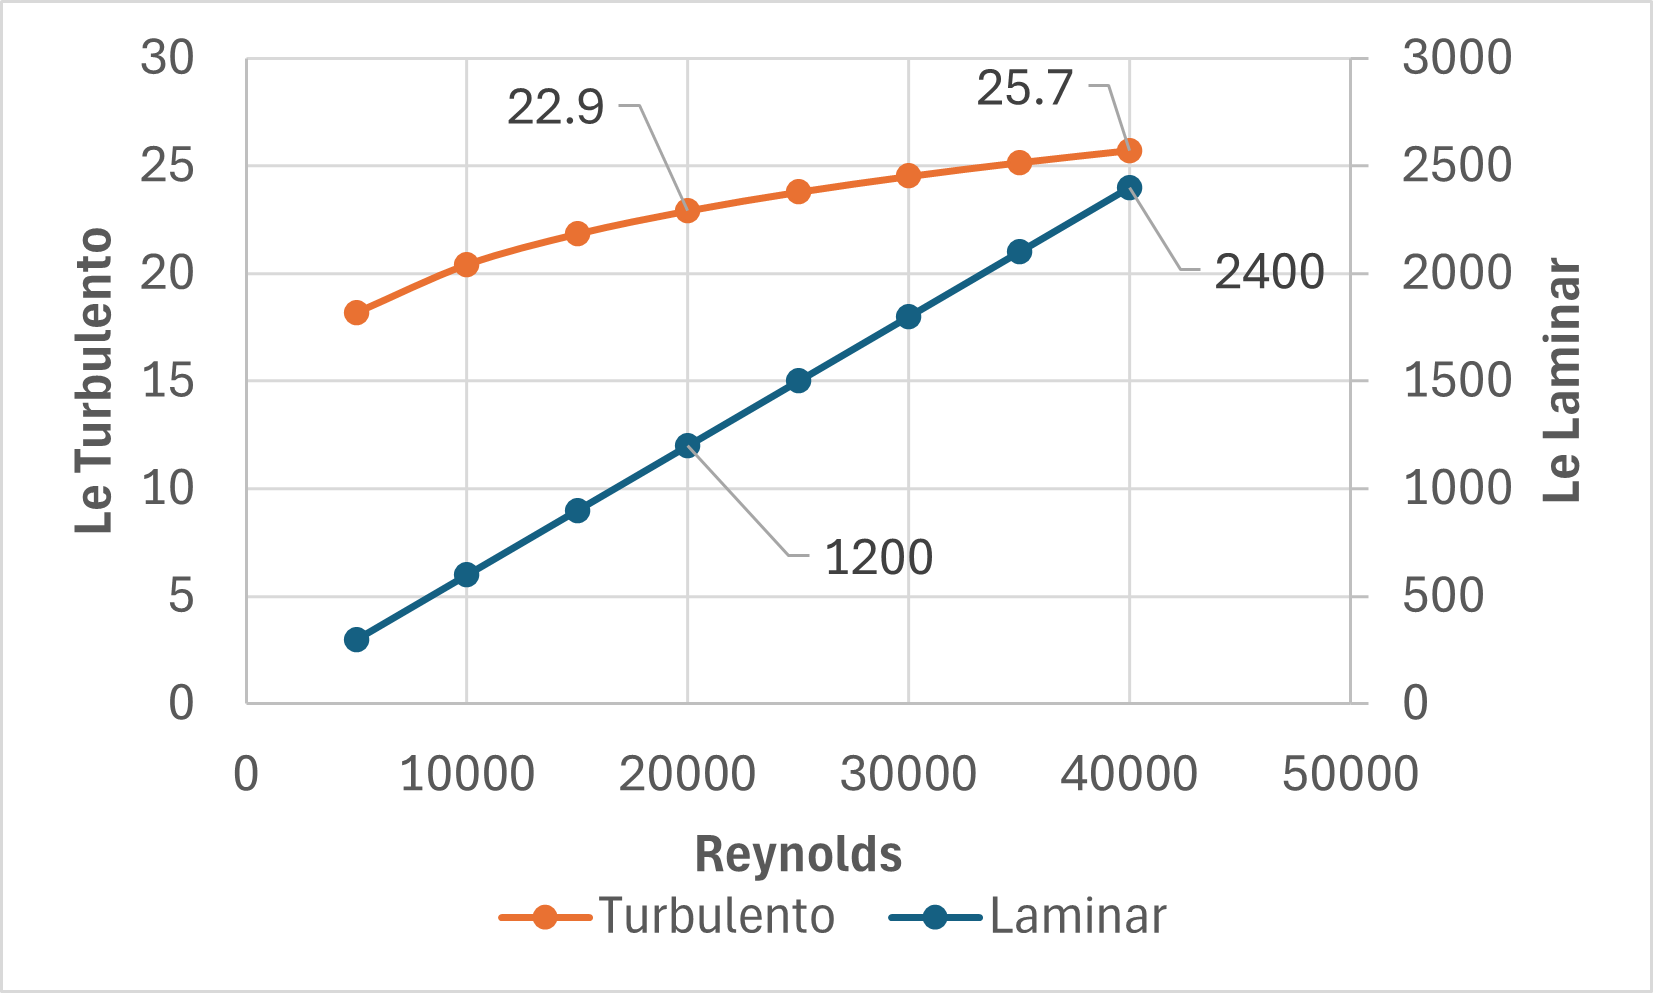
\includegraphics[width=.65\textwidth]{figures/4}
	\caption{Distribuição de $u$ em x = 0,5 malha 50x50 volumes}
\end{figure}

A Figura 3 mostra o comportamento da velocidade em x(u) ao longo da referida reta vertical. Percebe-se que a solução numérica não reproduz exatamente o perfil de referência, principalmente nos valores de 0,6 e , 1,0. Isto é justificado pelos erros associados à malha grosseira que podem causar estes desvios, em zonas onde o gradiente de velocidade é mais perceptível (neste caso, perto da tampa deslizante). Na Figura 4, a solução numérica está mais próxima da solução de referência com maior precisão. O refinamento da malha permite que as médias feitas pela discretização espacial gerem menos erros numéricos devido ao esquema de interpolação. \\

Fica evidente neste primeiro desenvolvimento que o sistema de acoplamento pressão-velocidade apresenta bom desempenho para resolução do campo de pressão, bem como a boa interpolação feita pelo sistema WUDS onde se espera resolver adequadamente o problema de baixa advecção.

\subsection*{Casos para o numero de Reynolds Re=1000}


\begin{figure}[H]
	\centering
	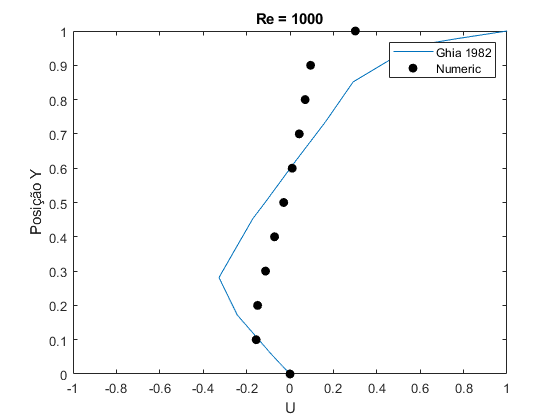
\includegraphics[width=.65\textwidth]{figures/5}
	\caption{Distribuição de $u$ em x = 0,5 malha 10x10 volumes}
\end{figure}

\begin{figure}[H]
	\centering
	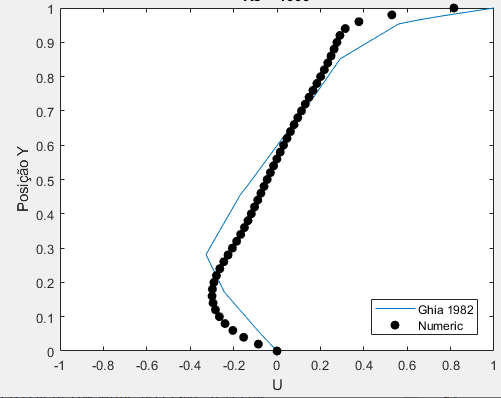
\includegraphics[width=.65\textwidth]{figures/6}
	\caption{Distribuição de $u$ em x = 0,5 malha 50x50 volumes}
\end{figure}

Com o aumento do número de Reynolds, o gradiente de velocidade muda. Uma diferença importante pode ser observada no limite inferior (y = 0) em relação ao caso de Re = 100. Para o caso da malha mais espessa de 10 x 10 volumes, o erro é maior que no caso anterior. O aumento dos fluxos advectivos deu indícios de necessidade de maior discretização espacial. Isto foi confirmado com os resultados mostrados na Figura 6, onde uma malha mais fina pode capturar melhor o gradiente de velocidade e, portanto, o erro em relação à referência é menor. No entanto, as diferenças nas fronteiras ainda são importantes.

\begin{figure}[H]
	\centering
	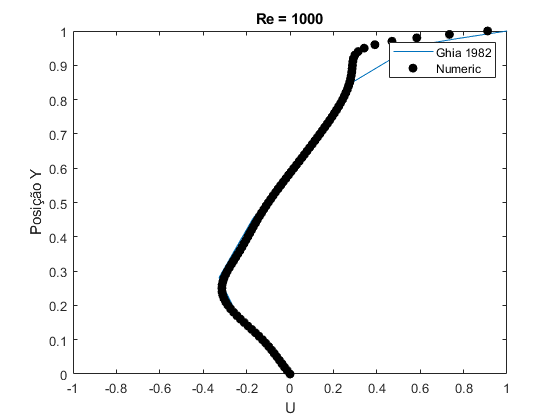
\includegraphics[width=.65\textwidth]{figures/8}
	\caption{Distribuição de $u$ em x = 0,5 malha 100x100 volumes}
\end{figure}

Uma melhor resolução do gradiente é obtida no caso da malha de volume 100 x 100. A previsão da curva de referência tem boa precisão, até y = 0,8. O problema do efeito de tampa deslizante próximo ao limite superior ainda apresenta erros significativos. Isto mostra que um refinamento local nesta área provavelmente funciona melhor do que um refinamento generalizado. Essa malha levou o maior tempo de solução para o problema numérico, por isso é importante dedicar efetivamente os refinamentos para preservar a eficiência e a precisão numérica.

\section*{Comentários finais e conclusões}

\begin{itemize}
	\item Este trabalho mostra a capacidade de ferramentas computacionais em prever problemas de mecânica dos fluidos. Especificamente, foi demonstrado que os esquemas de interpolação espacial e acoplamento do problema não linear de pressão e velocidade apresentam bom desempenho numérico para prever fluxos laminares com diferentes pesos de advecção e difusão.
	\item Os métodos descritos em [1], vistos ao longo da disciplina, são úteis para a previsão de um problema de fluido de referência [3] quando implementados em um sistema de solução de equações algébricas computacionais.
	\item Como esperado, o esquema de interpolação WUDS apresentou resultados com boa precisão para fluxos advectivos e difusivos.
	\item O esquema SIMPLE, embora tenha sido útil neste trabalho, depende de fatores de relaxação que estão longe dos problemas reais de mecânica dos fluidos.
	\item A importância prioritária da correta discretização do espaço ficou evidente quando os gradientes phi tiveram que ser resolvidos. Especialmente no caso de Re = 1000 onde os gradientes de velocidade nas fronteiras são maiores.
	
\end{itemize}

\textbf{\href{https://drive.google.com/file/d/1bugQAO7Zut6hmg514VoiJRC326zx53RL/view?usp=sharing}{Acceder ao codigo fazendo click aqui}}



\begin{thebibliography}{99}
	
	\bibitem{bookref} 
	Maliska,Clovis. 
	\textit{Transferência De Calor E Mecânica Dos Fluidos Computacional }. LTC, 2004.
	
	\bibitem{bookref} 
	H K Versteeg and W Malalasekera. 
	\textit{An Introduction
		to Computational
		Fluid Dynamics}. Pearson Education, 2007.
	
	\bibitem{articleref} 
	Ghia, U. Et al.
	"High-Re Solutions for Incompressible Flow
	Using the Navier-Stokes Equations and a
	Multigrid Method". \textit{Journal of Computational Physics} 1982.
	
	\bibitem{bookref} 
	Maliska,Clovis. 
	\textit{Transferência De Calor E Mecânica Dos Fluidos Computacional }. Springer, 2023.
	
\end{thebibliography}

\end{document}